\documentclass[10pt]{article}
\usepackage{mathpaper}
\usepackage{tabularx}
\begin{document}
\showsecret
\papertitle{第21$\boldsymbol{\sim}$23章综合能力提升卷}
\paperinformation
\begin{questions}{\selectingintroduction}
    \question 已知$a$是一个实数,则下列关于$x$的函数中,(~~~~~~~)一定是二次函数.
    \twp{$y=ax^2-x+1$}{$y=(x+1)(x-3)-(x+4)(x-8)$}{$y=(a^2-a+1)x^2+ax-a^2$}{$y=\left|a+1\right|x^2-7x+10a$}
    \question 一元二次方程$-3x^2-3x+5=0$的两根之和为(~~~~~~~).
    \onp{$-1$}{$1$}{$5$}{$-5$}
    \question 在平面直角坐标系中,点$(3,2)$关于原点的对称点是(~~~~~~~).
    \onp{$(3,-2)$}{$(-2,-3)$}{$(-3,-2)$}{$(-3,2)$}
    \question 如图,$\Delta ABC$与$\Delta AEF$均为等边三角形,连$BE$、$CF$,则下列结论不一定成立的是(~~~~~~~).
    \onp{$BE=CF$}{$\angle BAE=\angle CAF$}{$\angle EBC+\angle BCF=120^{\circ}$}{$BE=EF$}
    \question 已知抛物线$y=ax^2+ax-b \ (a < 0)$上有三点$(1,y_1)$、$(-1,y_2)$、$(-3,y_3)$,则$y_1$、$y_2$、$y_3$之间的大小关系正确的是(~~~~~~~).
    \onp{$y_2>y_3>y_1$}{$y_2>y_1>y_3$}{$y_1>y_2>y_3$}{$y_1>y_3>y_2$}
    \question 已知抛物线$C_1:y=2x^2-4x+1$,将$C_1$向上平移$3$个单位长度、向左平移$2$个单位长度可得到抛物线$C_2$,则抛物线$C_2$的解析式为(~~~~~~~).
    \onp{$y=2x^2+4x-2$}{$y=2x^2-12x+20$}{$y=2x^2+4x+4$}{$y=2x^2-12x+14$}
    \question 一座桥的桥洞形状为抛物线,当水位正常时,水面的宽度是桥洞顶点到水面距离的2倍,水上涨3米后,水面的宽度是正常时的一半,则正常时水面宽(~~~~~~~)米.
    \onp{$3$}{$4$}{$6$}{$8$}
    \question 如图,在等边三角形$ABC$内有一点$P$,连$AP$、$BP$、$CP$,若$AP=4$、$CP=3$、$\angle APC=150^{\circ}$,则线段$BP$长度为(~~~~~~~).
    \onp{$5$}{$3$}{$\sqrt{7}$}{$\sqrt{41}$}
    \question 已知两不等实数$m$、$n$满足$m^2-3m-1=0$、$n^2-3n-1=0$,则代数式$m^3-2m^2+n^2-\frac{1}{n}+2n$的值为(~~~~~~).
    \onp{$17$}{$-7$}{$-12$}{$12$}
    \question 如图,四边形$ABCD$和$AEFG$均是正方形,连$ED$、$BG$交于点$T$,点$K$是线段$BC$上一点,使得$CK=\frac{1}{8}BC=1$,连线段$TC$并取其中点$Q$,连$QK$,则线段$QK$长度的最大值是(~~~~~~~).
    \onp{$\sqrt{5}+2\sqrt{2}$}{$2\sqrt{5}$}{$\frac{1}{2}+\sqrt{2}$}{$\frac{\sqrt{2}}{2}+2\sqrt{5}$}
    \begin{figure}[!htb]
        \centering
        \subfigure[(第4题)]
        {
            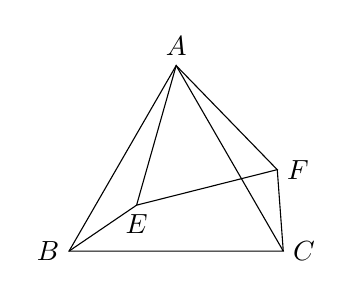
\begin{tikzpicture}[scale=0.5]
                \coordinate[label=above:{$A$}] (A) at (0,0);
                \coordinate[label=left:{$B$}] (B) at (-2.72061,-4.71224);
                \coordinate[label=right:{$C$}] (C) at (2.72061,-4.71224);
                \coordinate[label=below:{$E$}] (E) at (-1.00542,-3.54542);
                \coordinate[label=right:{$F$}] (F) at (2.56771,-2.64342);
                \draw (A) -- (B) -- (C) -- cycle;
                \draw (A) -- (E) -- (F) -- cycle;
                \draw (B) -- (E);
                \draw (C) -- (F);
            \end{tikzpicture}
        }\qquad\qquad\qquad
        \subfigure[(第8题)]{
            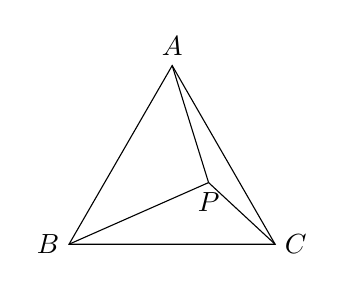
\begin{tikzpicture}[scale=0.65]
                \coordinate[label=above:{$A$}] (A) at (0,0);
                \coordinate[label=left:{$B$}] (B) at (-2.01501,-3.49009);
                \coordinate[label=right:{$C$}] (C) at (2.01051,-3.49009);
                \coordinate[label=below:{$P$}] (P) at (0.71105,-2.28594);
                \draw (A) -- (B) -- (C) -- cycle;
                \draw (P) -- (A);
                \draw (P) -- (B);
                \draw (P) -- (C);
            \end{tikzpicture}
        }\qquad\qquad\qquad
        \subfigure[(第10题)]{
            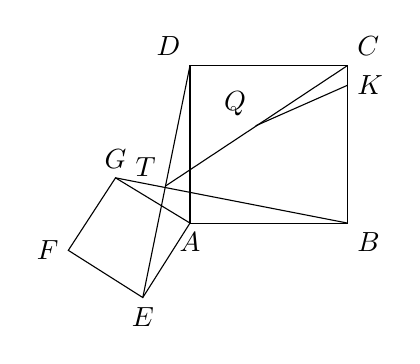
\begin{tikzpicture}[scale=0.25]
                \coordinate[label=below:{$A$}] (A) at (-8,0);
                \coordinate[label=below right:{$B$}] (B) at (0,0);
                \coordinate[label=above right:{$C$}] (C) at (0,8);
                \coordinate[label=above left:{$D$}] (D) at (-8,8);
                \coordinate[label=below:{$E$}] (E) at (-10.39812,-3.78354);
                \coordinate[label=left:{$F$}] (F) at (-14.18167,-1.38542);
                \coordinate[label=above:{$G$}] (G) at (-11.78354,2.29812);
                \coordinate[label=right:{$K$}] (K) at (0,7);
                \coordinate[label=above left:{$T$}] (T) at (-9.24520,1.88153);
                \coordinate[label=above left:{$Q$}] (Q) at (-4.66260,4.94077);
                \draw (A) -- (B) -- (C) -- (D) -- cycle;
                \draw (A) -- (E) -- (F) -- (G) -- cycle;
                \draw (D) -- (E);
                \draw (B) -- (G);
                \draw (K) -- (Q);
                \draw (C) -- (T);
            \end{tikzpicture}
        }
    \end{figure}
\end{questions}

\begin{questions}{\complitingintroduction}
    \question 抛物线$y=2x^2+4x-1$的顶点是\complitingline
    \question 在平面直角坐标系中,点$(3,7)$关于点$(0,1)$的对称点是\complitingline
    \question 若当$-3 \leq x \leq 2$时,函数$y=x^2+4x+a$的最小值与最大值之积为$-28$,则$a$的值为\complitingline
    \question 如图,在直角三角形$ABC$中,$\angle A=65^{\circ}$、$\angle ABC=90^{\circ}$.将$\Delta ABC$绕点$B$顺时针旋转至$\Delta DBE$处,使点$D$落在$AC$上.记$DE$与$BC$的交点为$K$,则$\angle CKE$的大小为\complitingline
    \begin{figure}[!htb]
        \raggedleft
        \subfigure[(第14题)]{
            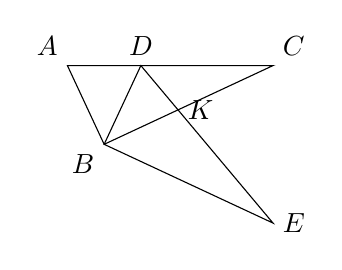
\begin{tikzpicture}[scale=0.5]
                \coordinate[label=above left:{$A$}] (A) at (-0.93262,2);
                \coordinate[label=below left:{$B$}] (B) at (0,0);
                \coordinate[label=above right:{$C$}] (C) at (4.28901,2);
                \coordinate[label=above:{$D$}] (D) at (0.93262,2);
                \coordinate[label=right:{$E$}] (E) at (4.28901,-2);
                \coordinate[label=right:{$K$}] (K) at (1.87656,0.87505);
                \draw (A) -- (B) -- (C) -- cycle;
                \draw (D) -- (B) -- (E) -- cycle;
            \end{tikzpicture}
        }
    \end{figure}
    \question 已知实数$a$、$b$、$c$满足$a+b+c=0$、$0 < 3a \leq c$,则有下列说法:
    \begin{subsubquestions}
        \subsubquestion $9a+3b+c \geq 0$.
        \subsubquestion $5a+2b+c \leq 0$.
        \subsubquestion 对任意的$x \geq 2$,不等式$ax^2+bx+c \geq 4a+2b+c$恒成立.
        \subsubquestion 若$16a+4b+c=3$,则关于$x$的不等式$ax^2+(b-1)x+c+1 \geq 0$的解集是$1 \leq x \leq 4$.
    \end{subsubquestions}
    其中正确的是\complitingline
    \question Pick定理是格点几何学中的重要定理,在平面直角坐标系中,格点指横、纵坐标均为整数的点.若记$N$为一多边形内部(不包括边上)格点的个数,$L$为该多边形边上格点的个数,$S$为该多边形的面积,则Pick定理为:$S=N+\frac{1}{2}L-1$.若在平面直角坐标系中有点$A(240,0)$、$B(180,40)$、$C(0,220)$、$D(60,200)$,则四边形$ABCD$内部(不包括边上)的格点数为\complitingline
\end{questions}

\begin{questions}{\answeringintroduction}
    \question 分别求下列抛物线的开口方向、顶点坐标以及与$x$轴的交点坐标:
    \begin{subquestions}
        \subquestion $y=x^2-8x+12$
        \subquestion $y=-2x^2+6x+8$
    \end{subquestions}
    \addemptyline\addemptyline\addemptyline\addemptyline
    \question 如图,$\Delta ABC$和$\Delta AEF$均为等边三角形,连$BE$、$CF$交于点$Q$.
    \begin{subquestions}
        \subquestion 求证:$BE=CF$.
        \subquestion 求$\angle BQF$.
    \end{subquestions}
    \begin{figure}[!htb]
        \raggedleft
        \subfigure[(第18题)]{
            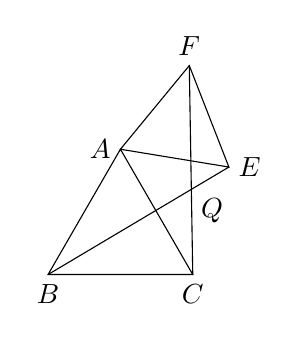
\begin{tikzpicture}[scale=0.45]
                \coordinate[label=left:{$A$}] (A) at (0,0);
                \coordinate[label=below:{$B$}] (B) at (-2.04146,-3.53592);
                \coordinate[label=below:{$C$}] (C) at (2.04146,-3.53592);
                \coordinate[label=right:{$E$}] (E) at (3.06125,-0.50271);
                \coordinate[label=above:{$F$}] (F) at (1.94348,2.36080);
                \coordinate[label=below right:{$Q$}] (Q) at (2.00118,-1.11147);
                \draw (A) -- (B) -- (C) -- cycle;
                \draw (A) -- (E) -- (F) -- cycle;
                \draw (B) -- (E);
                \draw (C) -- (F);
            \end{tikzpicture}
        }
    \end{figure}
    \question 在一个小区内,有一人患上了流感,经过两轮传染后,总共有$64$人患上了流感.
    \begin{subquestions}
        \subquestion 平均在每轮传染中,一个流感患者可以将流感传染给多少人?
        \subquestion 第二年流感再次来袭时,该小区采取了恰当的应对措施,每一个流感患者在传播完一轮后都被及时发现并被医治健康,并且流感在第三轮传染开始前被彻底消灭,若一开始只有一人患上流感,流感被消灭后累计31人在这一年得过流感,则这一年平均一个流感患者只将流感传染给了几个人?
    \end{subquestions}
    \newpage
    \question 已知关于$x$的一元二次方程$x^2+4x+m+1=0$有两个实数根$x_1$、$x_2$.
    \begin{subquestions}
        \subquestion 求实数$m$的取值范围.
        \subquestion 若${x_1}^2+{x_2}^2-4{x_1}{x_2}=0$,求实数$m$的值.
    \end{subquestions}
    \addspace
    \question 如图,在$8 \times 8$的网格中,点$A$、$B$、$C$均是格点,且以这三点围成的三角形是以$B$为直角顶点的直角三角形.仅用无刻度直尺完成下列作图任务(保留作图痕迹):
    \begin{subquestions}
        \subquestion 在图1中,作$\angle BCA$的角平分线.
        \subquestion 在图2中,点$T$是线段$AC$上的任意一点,在线段$AB$上作点$E$,使得$EA=TA$.
        \subquestion 在(2)的条件下,记$\angle BAC=\alpha$,将点$T$绕点$A$逆时针旋转$\alpha$至点$F$,求作点$F$.
    \end{subquestions}
    \begin{figure}[!htb]
        \centering
        \subfigure[(1)]{
            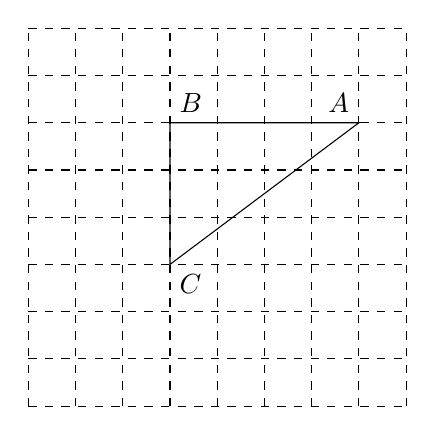
\begin{tikzpicture}[scale=0.6]
                \draw[step=1,dashed] (-3,-3) grid (5,5);
                \coordinate[label=below right:{$C$}] (C) at (0,0);
                \coordinate[label=above left:{$A$}] (A) at (4,3);
                \coordinate[label=above right:{$B$}] (B) at (0,3);
                \draw (A) -- (B) -- (C) -- cycle;
            \end{tikzpicture}}\qquad\qquad
        \subfigure[(2)]{
            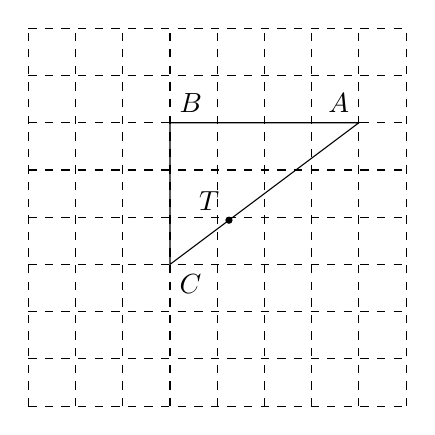
\begin{tikzpicture}[scale=0.6]
                \draw[step=1,dashed] (-3,-3) grid (5,5);
                \coordinate[label=below right:{$C$}] (C) at (0,0);
                \coordinate[label=above left:{$A$}] (A) at (4,3);
                \coordinate[label=above right:{$B$}] (B) at (0,3);
                \coordinate[label=above left:{$T$}] (T) at (1.24848,0.93636);
                \filldraw (T) circle (0.064);
                \draw (A) -- (B) -- (C) -- cycle;
            \end{tikzpicture}
        }
        \caption*{(第21题)}
    \end{figure}
    \question 在一次军事演习中,我军一架无人机正在以$100$m/s的飞行速度与$500$m的飞行高度对一片山区执行低空轰炸任务,已知该飞机以水平轰炸的方式投下航空炸弹,且炸弹的下落距离$h$、水平飞行距离$x$和飞行时间$t$之间的关系如下表所示(不计空气阻力):
    \begin{figure}[!htb]
        \centering
        \subfigure{
            \begin{tabularx}{0.5\textwidth}[!htb]{|m{3.8cm}<{\centering}|*{4}{>{\centering\arraybackslash}X|}} \hline
                飞行时间$t$(s)& 0 & 1 & 2 & 3 \\ \hline
                水平飞行距离$x$(m)& 0 & 100 & 200 & 300 \\ \hline
                下落距离$h$(m) & 0 & 5 & 20 & 45 \\ \hline
            \end{tabularx}
        }
        \subfigure{
        \begin{tikzpicture}[>=Stealth,scale=0.5]
            \draw[->] (-7.5,0) -- (4.2,0) node[below] {$x$};
            \draw[->] (0,-1) -- (0,5.5) node[right] {$y$};
            \coordinate[label=below right:{$O$}] (O) at (0,0);
            \draw (0,0) -- (3.5,3.5) -- (4.2,3.5);
            \draw (-7,5) parabola bend (-7,5) (1.5,1.5);
            \filldraw (-7,5) circle (.1);
            \node[below] at (-7,5) {无人机};
            \draw[line width =2pt] (1,1) -- (2,2);
        \end{tikzpicture}}
    \end{figure}
    \par 其中,$x$与$t$和$h$与$t$之间存在函数关系,且这些函数都是我们学过的函数.
    \begin{subquestions}
        \subquestion 直接写出$x$与$t$和$h$与$t$之间的函数关系式(不必写出$t$的取值范围).
        \subquestion 已知无人机攻击的目标在一座坡度为$45^{\circ}$的山处,现以山脚为原点,建立如图所示的坐标系.
        \begin{subsubquestions}
            \subsubquestion 在一次投弹任务中,已知航弹释放后正好在无人机从山脚正上方掠过时落地爆炸,求投弹点与山脚间的水平距离.
            \subsubquestion 已知在山坡上水平距离山脚$100$m至$200$m的地方(包括这两点,图中已经加粗)有敌军的迫击炮阵地,若无人机需要攻击那里,求无人机与山脚之间水平距离的取值范围.
        \end{subsubquestions}
    \end{subquestions}
    \newpage
    \question %23
    \begin{subquestions}
        \subquestion 已知等边三角形$ABC$内(不包括三边)有一点$P$.
        \begin{subsubquestions}
            \subsubquestion 如图1,连$PB$、$PC$,求证:$PB+PC<2BC$.
            \subsubquestion 如图2,连$PC$,以$PC$为边,向外作菱形$CPEQ$,使$\angle PCQ=60^{\circ}$,连$BE$并取其中点$F$,连$AF$、$PF$.试求出线段$AF$与线段$PF$之间的关系.
        \end{subsubquestions}
        \subquestion 如图3,在凹四边形$ABCD$中,连$BD$,有$\angle ADB=120^{\circ}$、$\angle CDB=105^{\circ}$,将线段$AB$绕点$B$顺时针旋转$150^{\circ}$得到线段$TB$,连$CT$,若$AD+BD=7$、$CD=1$,直接写出线段$CT$长度的最小值.
    \end{subquestions}
    \begin{figure}[!htb]
        \centering
        \subfigure[(1)]{
        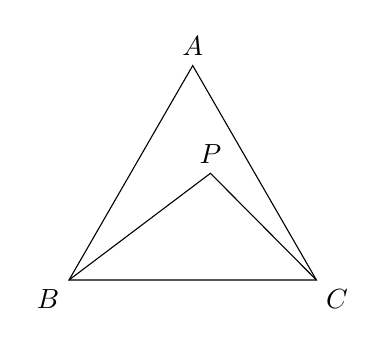
\begin{tikzpicture}[scale=0.45]
            \coordinate[label=above:{$A$}] (A) at (3.49,6.05);
            \coordinate[label=below left:{$B$}] (B) at (0,0);
            \coordinate[label=below right:{$C$}] (C) at (6.98,0);
            \draw (A) -- (B) -- (C) -- cycle;
            \coordinate[label=above:{$P$}] (P) at (3.99,3.01);
            \draw (B) -- (P) -- (C);
        \end{tikzpicture}}\qquad
        \subfigure[(2)]{
        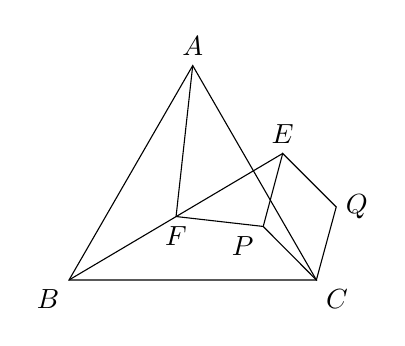
\begin{tikzpicture}[scale=0.45]
            \coordinate[label=above:{$A$}] (A) at (3.49,6.05);
            \coordinate[label=below left:{$B$}] (B) at (0,0);
            \coordinate[label=below right:{$C$}] (C) at (6.98,0);
            \draw (A) -- (B) -- (C) -- cycle;
            \coordinate[label=below left:{$P$}] (P) at (5.48,1.51);
            \coordinate[label=right:{$Q$}] (Q) at (7.54,2.06);
            \coordinate[label=above:{$E$}] (E) at (6.03,3.57);
            \coordinate[label=below:{$F$}] (F) at (3.02,1.79);
            \draw (P) -- (C) -- (Q) -- (E) -- cycle;
            \draw (B) -- (E);
            \draw (A) -- (F) -- (P);
        \end{tikzpicture}}\quad
        \subfigure[(3)]{
        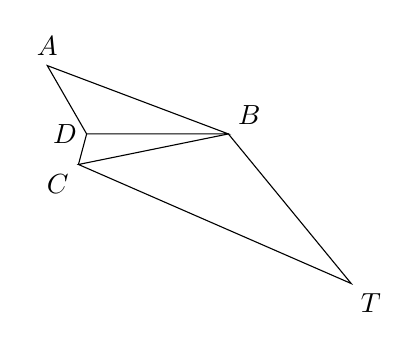
\begin{tikzpicture}[scale=0.4]
            \coordinate[label=above:{$A$}] (A) at (-1.25,2.17);
            \coordinate[label=above right:{$B$}] (B) at (4.5,0);
            \coordinate[label=below left:{$C$}] (C) at (-0.26,-0.97);
            \coordinate[label=left:{$D$}] (D) at (0,0);
            \coordinate[label=below right:{$T$}] (T) at (8.40,-4.75);
            \draw (A) -- (D) -- (B) -- cycle;
            \draw (B) -- (C) -- (T) -- cycle;
            \draw (C) -- (D);
        \end{tikzpicture}}
        \caption*{(第23题)}
    \end{figure}
    \question 在平面直角坐标系$xOy$中,抛物线$y=x^2-2x-3$的顶点是$D$,交$x$轴于点$A$、点$B$(点$A$在点$B$左侧),交$y$轴于点$C$.
    \begin{subquestions}
        \subquestion 直接写出点$A$、点$B$、点$C$、点$D$的坐标.
        \subquestion 如图1,连$BC$,设直线$l_1:x=t$交线段$BC$(含两端)于点$E$,交抛物线于点$F$,直线$l_2:x=t+1$交线段$BC$(含两端)于点$M$,交抛物线于点$N$,试根据$t$的取值讨论线段$EF$与线段$MN$的大小关系.
        \subquestion 如图2,过点$(2,-2)$的直线交抛物线于点$P$、$Q$,作直线$PB$与直线$DQ$交于点$T$,连$AT$,求线段$AT$长度的最小值.
    \end{subquestions}
    \begin{figure}[!htb]
        \centering
        \subfigure[(1)]{
            \begin{tikzpicture}[>=Stealth,scale=0.8]
                \draw[->] (-2,0) -- (5,0) node[below] {$x$};
                \draw[->] (0,-5) -- (0,2) node[right] {$y$};
                \coordinate[label=below right:{$O$}] (O) at (0,0);
                \draw (-1.24,1) parabola bend (1,-4) (3.24,1);
                \coordinate[label=below left:{$A$}] (A) at (-1,0);
                \coordinate[label=below right:{$B$}] (B) at (3,0);
                \coordinate[label=left:{$C$}] (C) at (0,-3);
                \draw (B) -- (C);
                \draw (0.8,-5) -- (0.8,2);
                \coordinate[label=left:{$E$}] (E) at (0.8,-2.2);
                \coordinate[label=left:{$F$}] (F) at (0.8,-3.96);
                \draw (1.8,-5) -- (1.8,2);
                \coordinate[label=left:{$M$}] (M) at (1.8,-1.2);
                \coordinate[label=left:{$N$}] (N) at (1.8,-3.36);
            \end{tikzpicture}
        }\qquad\qquad
        \subfigure[(2)]{
            \begin{tikzpicture}[>=Stealth,scale=0.8]
                \draw[->] (-2,0) -- (5,0) node[below] {$x$};
                \draw[->] (0,-5) -- (0,2) node[right] {$y$};
                \coordinate[label=below right:{$O$}] (O) at (0,0);
                \draw (-1.24,1) parabola bend (1,-4) (3.24,1);
                \coordinate[label=below left:{$A$}] (A) at (-1,0);
                \coordinate[label=below right:{$B$}] (B) at (3,0);
                \coordinate[label=below:{$D$}] (D) at (1,-4);
                \draw (-1.52,-1.22) -- (4.46,-2.54);
                \coordinate[label=below:{$P$}] (P) at (-0.60,-1.43);
                \coordinate[label=below right:{$Q$}] (Q) at (2.38,-2.08);
                \draw (-1.51,-1.79) -- (4.80,0.71);
                \draw (0.54,-4.64) -- (4.76,1.20);
                \coordinate[label=below right:{$T$}] (T) at (4.25,0.49);
                \draw (A) -- (T);
            \end{tikzpicture}
        }
        \caption*{(第24题)}
    \end{figure}
\end{questions}
\end{document}